\documentclass[a4paper, titlepage, 12pt]{article}
\usepackage{graphicx}
\usepackage{color}
\usepackage{hyperref}
\usepackage{amsmath}
\usepackage{amsthm}
\usepackage{adjustbox}
\usepackage{float}
\usepackage{mdframed}
\usepackage{subfig}
\usepackage[T1]{fontenc}
\DeclareMathOperator{\argmax}{arg\,max}
\numberwithin{equation}{section}
% For box
\usepackage{collectbox}

\makeatletter
\newcommand{\mybox}{%
    \collectbox{%
        \setlength{\fboxsep}{1pt}%
        \fbox{\BOXCONTENT}%
    }%
}
\makeatother
%Endfor box



\begin{document}
    \title{ECE - 5534 Electronic Design Automation \\ ROBDDs}
    \author{Prathamesh Mandke \\ \href{pkmandke@vt.edu}{pkmandke@vt.edu} \\ PID: 906239574}
    \date{\today \\ \href{https://ece.vt.edu}{ECE} @ \href{https://vt.edu}{Virginia Tech}}
    \maketitle
    \newpage

    \section{Lab Overview}

        Reduced Ordered Binary Decision Diagrams (ROBDDs) are concise representations of boolean expressions in the form of directed acyclic graphs.
        ROBDDs make use of the if-then-else (INF) form of boolean expressions to construct the graphical representation.
        An INF form of a boolean expression is one where any operations are only perfomed on variables combined with constants and other (recursive) INF statements.
        The practicality of using the INF form to construct ROBDDs for any boolean expression stems from the Shannon Expansion idea.
        Shannon Expansion involves breaking down an expression (with arbitrary number of variables) into an INF form by recursively setting and resetting the value of one variable at a time.
        From the perspective of implementation in digital logic, the Shannon Expansion involves cascading multiplexer circuits by considering all combinations of a boolean variable at a time.
        
        When a complicated boolean expression is recursively broken down into it's INF, a series of INF statements are obtained.
        Now, if any redundant INF statements are combined, the resulting set of INF statements can be expressed as a binary decision diagram (BDD).
        When the order of variable selection is same across all recursive builds of the INF forms, the resulting decision diagram has nodes in the same order starting from the root.
        Such a BDD is said to be an ordered BDD.
        Going one step further, multiple nodes with the same left and right nodes can be combined since they are obviously redundant.
        Such reduction leads to a unique representation of the boolean expression known as the ROBDD.

        This work involves the implementation of a ROBDD for boolean operations AND, OR, NOT, IMPLICATION and EQUIVALENCE.
        The methods used to implement the ROBDD have been inspired from Henrik Anderson's document on Binary Decision Diagrams.
        Specifically, the Build, Mk, Apply, Restrict, AllSat, StatCount and AnySat methods have been implemented.
        Build and Mk together make sure that the resulting BDD is in the reduced form.
        Apply combined the ROBDDs of 2 different expressions into a single ROBDD.
        Restrict constrains the ROBDD of a given expression by subsitituting for the values of certain variables.
        AllSat, Anysat and StatCount repectively return all the satisfying truth assignments, any one (arbitrary) truth assignment and the total number of truth assignments.
         
    \section{Code Structure}

        The ROBDD program has been implemented using the Python programming language.
        The main program accepts the expression as a command-line argument.
        Note that the input expression is not checked for correctness or balanced brackets.
        The input expression is first handled by a simple Lexical Analyzer to separate variables, functions and constants.
        Further, a Recursive Descent Parser (RDP) builds a tree from the lexical analyzers parsing output by quering the lexical analyzer.
        The expression API then recursively travels the RDP to compute/solve the boolean expression.
        
        The main classes and utilities in the codebase have been elucidated below.
        
        \begin{itemize}
            \item[1.] \textbf{robdd.py}
                
                This file defines the main \textbf{ROBDD} class that consists of the methods \textbf{Build, Mk, AnySat, AllSat and StatCount}.
                The ROBDD takes in the expression along with the number of variables as input while instantiation.
                
            \item[2.] \textbf{parsing.py}
            
                This file defines 3 important classes for handling the input expression.
                
                \textbf{Class Options:} Handles commandline arguments.
                
                \textbf{Class Lexer:} The Lexical Analyzer that reads the expression from the commandline and gets them ready for consumption by the RecursiveDescentParser class.

                \textbf{Class RecursiveDescentParser:} This class builds an expression tree and provides a method to traverse it.

            \item[3.] \textbf{expression.py}
            
                The \textbf{Expression class} in this file stands as a unified API for different of expression formats.
                Particularly, it can handle expression with or without the RecursiveDescentParser.
                Although, this functionality is now deprecated since the RecursiveDescentParser is intuitive and easy to use.
                Thus, the use\_rdp flag can be ignored.

            \item[4.] \textbf{utils.py}
            
                In addition to common utilities, this file defines the \textbf{Apply} and \textbf{Restrict} utilities as functions.
                This file also defines a \textbf{RDP\_node} class, which defines a node in a RecursiveDescentParser.
            
            \item[5.] \textbf{wrapper.py}
            
                The \textbf{Wrapper class} in this file provides a unifies API to using and testing various functionalities of the other classes.
                Importantly, it abstracts away the instantiation of all the aforementioned classes and handles the same with intuitive methods.
                It begins by accepting commandline arguments by instantiating the Options class from parsing.py and instantiating the Lexer, the RecursiveDescentParser, the Expression and one or more ROBDDs as needed.

            \item[6.] \textbf{main.py}
            
                The main program instantiates the Wrapper class and performs any required functions.
                The main program needs to be invoked with appropriate commandline parameters.
                Below are the commandline options, all of which are optional.

                nvars: int -> The maximum number of variables in the main expression.
                
                expr: str -> The main boolean expression as astring. Eg: --expr "equiv(imp(not(x1), and(x2, x3)), x3)"
                
                nvars1: int -> The maximum number of variables in expression 1. (Used by Apply as the first of two ROBDDs to be combined.)
                
                expr1: int -> The first of two expressions used by Apply to combine.
                
                nvars1: int -> The maximum number of variables in expression 2. (Used by Apply as the second of two ROBDDs to be combined.)
                
                expr1: int -> The second of two expressions used by Apply to combine.
                
                op: str -> The operation used by Apply to combine expr1 and expr2.
                
                j: int -> The variable number to be restricted with Restrict.
                
                b: int -> The value the variable x[j]. Must be either 0 or 1.
                
                call: str -> Name of the function defined in main.py that should be called on invoking main.py with the above command line parameters.

                A typical invokation could be:

                python3 main.py --nvars 2 --expr "and(x1, x2)" --nvars1 2 --expr1 "or(x1, x2)" --nvars 2 "not(x2)" --op "or" --j 2 --b 1 --call test\_time\_checks

        \end{itemize}
        

    \section{Tests}

        This section involves multiple tests and their results for verifying the functionality.
        Initially, I have considered simple unit tests for verifying the correctness of individual methods such as Build, Apply, etc. 
        Further, there are somewhat non-trivial and nuanced test cases for demonstrating the usefulness, simplicity and effectiveness of ROBDDs.

        \subsection{Unit Tests}

            This section includes unit tests for verifying functionality of individual methods of the ROBDD implementation.

            \begin{itemize}
                \item[1.] \textbf{Build (and Make)}
                    
                    It was difficult to find online utilities that could generate the T table for a given expression.
                    Thus, I have attempted to verify the same example as in the Henrik Anderson's document.
                    The expression in the document is "and(equiv(x1, x2), equiv(x2, x3))".

                    \begin{figure}[htp]
                        \centering
                        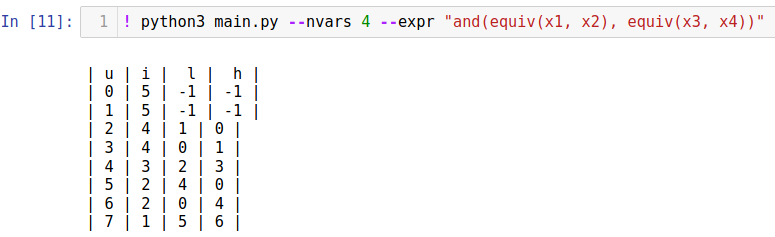
\includegraphics[height=0.3\textwidth, width=\textwidth]{img/robdd_build.png}
                        \caption{Program output}
                        \label{fig:build_prog_out}
                    \end{figure}
                    
                    \begin{figure}[htp]
                        \centering
                        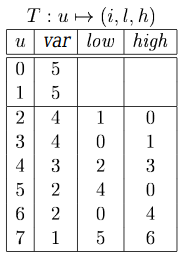
\includegraphics[height=140px, width=180px]{img/true_T_build.png}
                        \caption{True output}
                        \label{fig:build_true_out}
                    \end{figure}

                    The fact that the resulting BDD is also in the reduced form verifies the functionality of the Make (Mk) function as well.
                \item[2.] \textbf{Apply}
                    
                    Consider Figure \ref{fig:test_apply}.

                    \begin{figure}[htp]
                        \centering
                        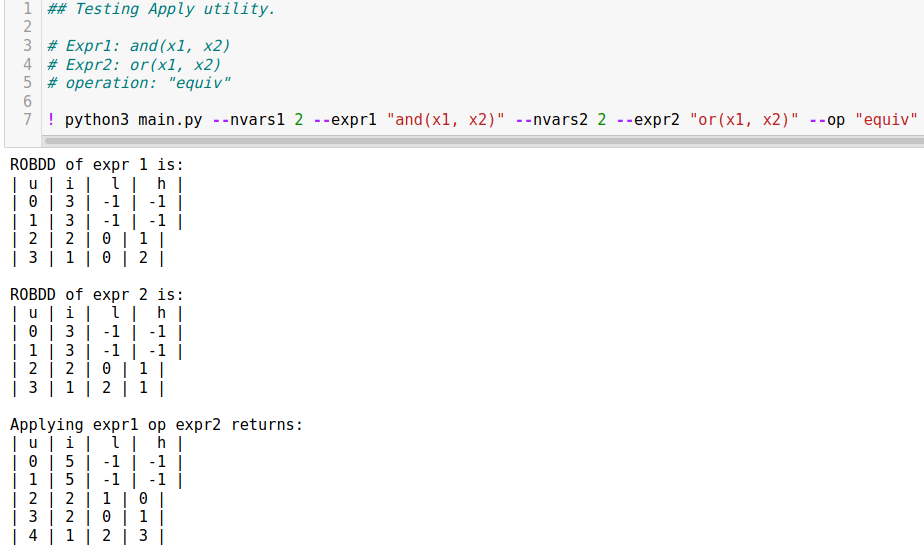
\includegraphics[height=250px, width=400px]{img/test_apply.png}
                        \caption{Testing Apply utility.}
                        \label{fig:test_apply}
                    \end{figure}

                    It is easy to observe that for the resulting expression "equiv(and(x1, x2), or(x1, x2))" the T table is correct.
                    Starting from the root node number 4, if $x1 = 0$ we check node 2 and if $x1 = 1$ we check node 3.
                    Now, if $x1 = 0$ then $and(x1, x2) = 0$ and the equivalence will only be true if $or(x1, x2)$ is true, that is, if $x2 = 1$.
                    This is verified from row with $u = 3$ of the resulting T table obtained after applying the equiv operation.
                    Similarly, the behaviour for $x1 = 1$ can be verified easily.

                \item[3.] \textbf{Restrict}

                    To verify that restrict works as intended, consider the expression not(or(and(x1, x2), equiv(x3, x4))).
                    Figure \ref{fig:test_restrict}, contains the results of restricting the variables $x1$, $x3$ and $x4$.

                    \begin{figure}[htp]
                        \centering
                        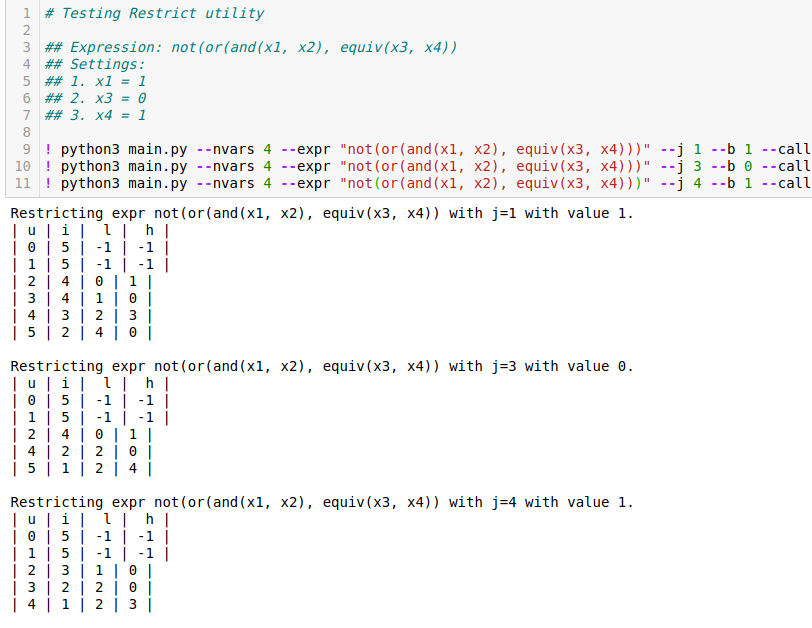
\includegraphics[height=250px, width=350px]{img/test_restrict_1.png}
                        \caption{Testing Restrict utility.}
                        \label{fig:test_restrict}
                    \end{figure}

                    For $x1 = 1$, we start from the root node $u = 5$, that is, we check $x2$.
                    Now if $x2 = 1$, clearly the OR condition is satisfied and the result is 0 due to the NOT.
                    If $x2 = 0$, we jump to node $u = 4$ and check x3.
                    Nodes $u = 2$, $u = 3$ and $u = 4$ capture the inverse of the logic of the EQUIV statement between x3 and x4.
                    The inverse is due to the outer NOT operator.

                    Similarly, the logic for $x3 = 0$ and $x4 = 1$ can be easily verified.
                    % It can be observed that when $x1 = 0$, the expression is 0 if x2 is 0 else it is 1.
                    % Moreover, if $x1 = 1$, the expression is 0 if x2 is 0 else it is 1.
                    % With $x2 = 0$, the expression will always be 0 while if $x2 = 1$ the expression is a tautology.
                    % In the last 2 cases, the root of the ROBDD changes although the T table looks alike.

                \item[4.] \textbf{StatCount, AnySat and AllSat}
                
                    Until now, I have considered relatively trivial examples since it was difficult to obtain T tables to compare and verify correctness.
                    However, for the statistical measures, the University of Utah provides a BDD interface for result verification at \href{http://formal.cs.utah.edu:8080/pbl/BDD.php}{this URL [1]}.

                    Consider the expression \textbf{not(or(and(equiv(x1, x2), equiv(x3, x4)), or(equiv(imp(x1, x5), imp(x4, x6)), and(x3, x7))))} which I made up randomly.

                    \begin{figure}[htp]
                        \centering
                        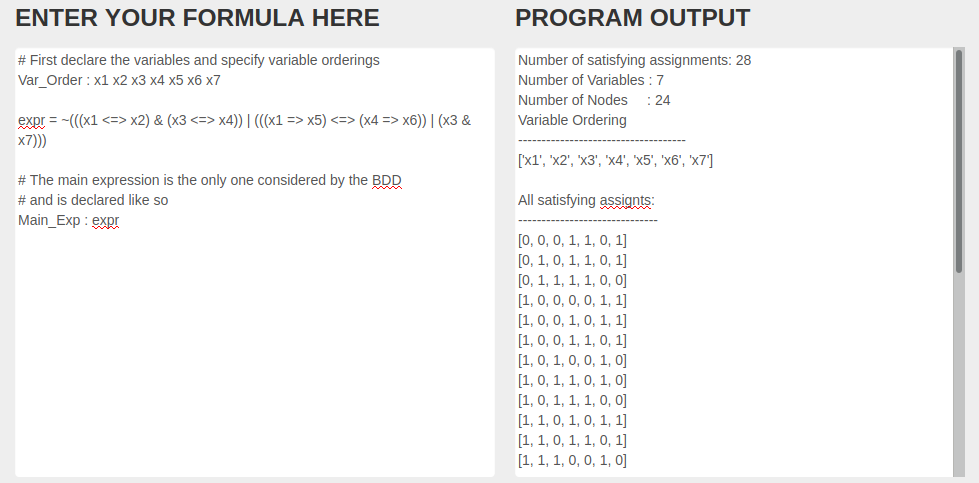
\includegraphics[height=200px, width=350px]{img/test_stats_true_1.png}
                        \caption{Statistics True Output 1.}
                        \label{fig:test_stats_true_1}
                    \end{figure}

                    \begin{figure}[htp]
                        \centering
                        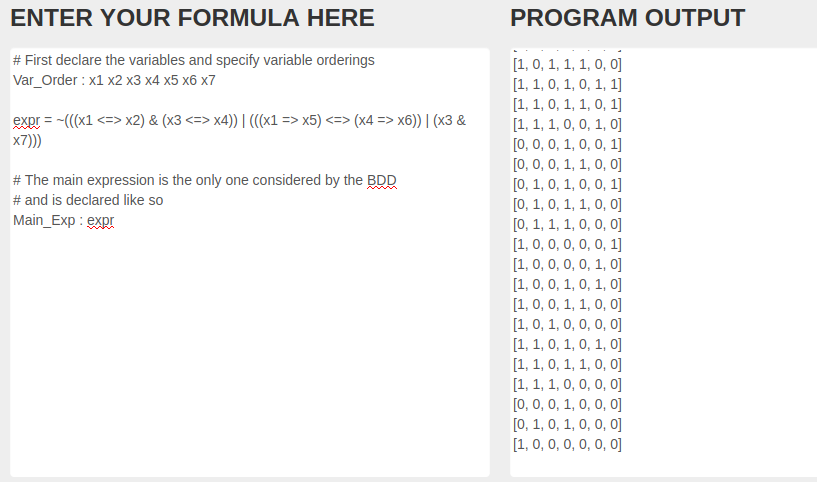
\includegraphics[height=200px, width=350px]{img/test_stats_true_2.png}
                        \caption{Statistics True Output 2.}
                        \label{fig:test_stats_true_2}
                    \end{figure}

                    \begin{figure}[htp]
                        \centering
                        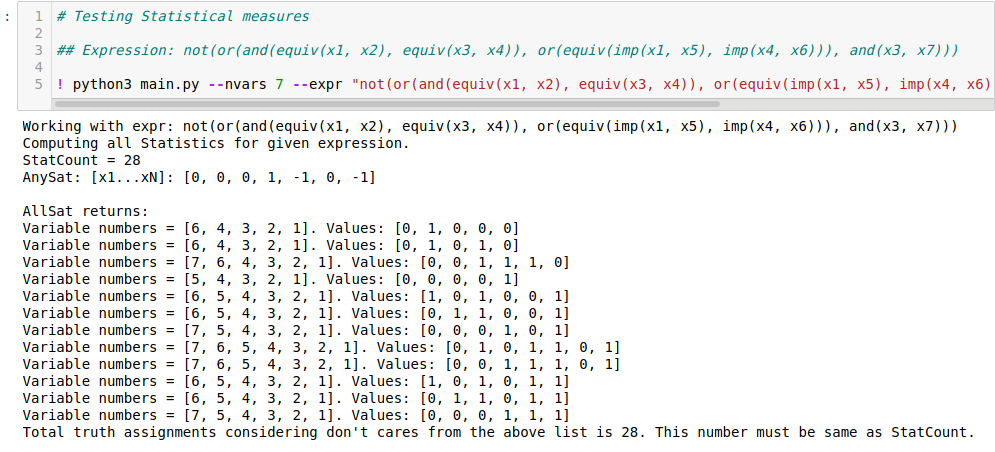
\includegraphics[height=200px, width=350px]{img/test_stats.png}
                        \caption{Testing Stats utilities.}
                        \label{fig:test_stats}
                    \end{figure}

                    Figure \ref{fig:test_stats_true_1} demonstrates the true results using \href{http://formal.cs.utah.edu:8080/pbl/BDD.php}{[1]}.
                    Figure \ref{fig:test_stats} shows the results of my program.
                    It can be verified that the number of satisfying assignments is 28 in both the cases.

                    Further \ref{fig:test_stats_true_2} shows the remaining of all the true satisfying assignments from using [1].
                    The program returns \[0,0,0,1,-1,0,-1\] as a possible satisfying assignment.
                    The -1's indicate don't cares.
                    Thus, in effect, this implies 4 different truth assignments.
                    From Figure \ref{fig:test_stats_true_1} and Figure \ref{fig:test_stats_true_2}, it can be seen that all 4 assignments that is [0,0,0,1,0,0,0], [0,0,0,1,0,0,1], [0,0,0,1,1,0,0], and [0,0,0,1,1,0,1] are a part of the truth assignment list.

                    For AllSat, the program output in Figure \ref{fig:test_stats} shows a set of unique truth assignments without considering don't cares.
                    Thus, it is not immediately obvious whether all assignments are being shown.
                    To verify this, I have written a simple script to exhaustively search and count all combinations of don't care assignments (of those variables that aren't a part of var\_idx).
                    Clearly, this count must equal the output of StatCount for the output of AllSat to be correct.
                    Both values are observed to be 28.


            \end{itemize}

        \subsection{Rutime Analysis}
            
            Consider the expression from the previous section \textbf{not(or(and(equiv(x1, x2), equiv(x3, x4)), or(equiv(imp(x1, x5), imp(x4, x6)), and(x3, x7))))}.
            In order to study time consumption by the program, I have increased the (maximum) number of variables in this expression.
            Since methods like build exhaustively search for path of all combinations of variables, the runtime analysis is expected to show a relatively sharp increasing trend.

            \begin{table}[H]
                \centering
                \caption{Time analysis (All values in seconds).}
                \label{tab:time_analysis}
                \begin{tabular}{|c|c|}
                    \hline \textbf{Maximum Variables} & \textbf{Build and Mk Time} \\ \hline
                    \textbf{7} & 0.000978s \\ \hline
                    \textbf{10} & 0.006462s \\ \hline
                    \textbf{12} & 0.026108s \\ \hline
                    \textbf{15} & 0.205158s \\ \hline
                    \textbf{20} & 6.831364s \\ \hline
                    \textbf{22} & 28.956934s \\ \hline
                    \textbf{25} & 03m48.974962s \\ \hline
                    % \textbf{Apply} & 0.000133s & 0.000134s & 0.000157s & 0.000134s\\ \hline
                    % \textbf{Restrict} & 0.000570s & 0.000086s & 0.000150s & 0.000083s \\ \hline
                    % \textbf{StatCount} & 0.000098s & 0.000067s & 0.000070s & 0.000071s \\ \hline
                    % \textbf{AnySat} & 0.000031s & 0.000008s & 0.000009s & 0.000009s \\ \hline
                    % \textbf{AllSat} & 0.000060s & 000041s & 0.000061s & 0.000043s\\ \hline
                \end{tabular}
            \end{table}

            Please refer to Table \ref{tab:time_analysis} for time runtime details of Build (and implicitly that of Mk).
            For verifying Build and Mk, I have used the aforementioned expression and increased the maximum variable count as shown in Table \ref{tab:time_analysis}.
            It can be observed that the runtime increases almost exponentially as the maximum number of variables in the expression increase.
            Since Build exhaustively traverses the path of all combinations of variables, the time is exponential in the number of variables.
            It is interesting to observe that merely increasing the number of variables (without including them in the expression) does not affect the time taken by any of the other methods such sa Apply, Restrict, etc.

            This is due to the fact that the other methods do not depend on the maximum number of variables but rather on the number of nodes in the ROBDD.
            Thus, in order to study their runtime, I consider the following increasing complex expressions in terms of the number of nodes in their ROBDDs and not just the maximum number of variables.
            
            \begin{itemize}
                \item[1.] \textbf{Apply}
                    
                    Table \ref{tab:apply_analysis} shows the time taken by Apply utility in combining two expressions.
                    The table consists of results from 2 runs with expressions of different sizes to be combined with the OR operator.
                    The runtime is proportional to the product of the number of nodes in the expressions to be combined.
                    
                    \begin{table}[!tbh]
                        \centering
                        \caption{Time analysis of Apply.}
                        \label{tab:apply_analysis}
                        \resizebox{\textwidth}{!}{\begin{tabular}{|c|c|c|}
                            \hline
                            \textbf{Run} & 1 & 2 \\ \hline
                            \textbf{Expression1} & and(equiv(x1, x2), equiv(x3, x4)) & equiv(x7, x4)\\ \hline
                            \textbf{Expression2} & or(equiv(imp(x1, x5), imp(x4, x6)), and(x3, x7)) & and(x3, x7) \\ \hline
                            \textbf{Operator} & OR & OR \\ \hline
                            \textbf{\# of nodes in expr1} & 8 & 5 \\ \hline
                            \textbf{\# of nodes in expr2} & 18 & 4\\ \hline
                            \textbf{Time} & 0.000127s & 0.000044s\\ \hline
                        \end{tabular}}
                    \end{table}


                \item[2.] \textbf{Restrict, AnySat, AllSat and StatCount}
                
                    To verify Restrict, AnySat and StatCount, I consider the following two expressions with different number of nodes in their ROBDDs.
                    Refer to Table \ref{tab:restrict_etal_analysis}.
                    
                    \begin{table}[!tbh]
                        \centering
                        \caption{Time analysis of Restrict, AnySat, AllSat and StatCount.}
                        \label{tab:restrict_etal_analysis}
                        \resizebox{\textwidth}{!}{\begin{tabular}{|c|c|c|}
                            \hline
                            \textbf{Run} & 1 & 2 \\ \hline
                            \textbf{Expression} & not(or(and(equiv(x1, x2), equiv(x3, x4)), or(equiv( \\ & imp(x1, x5), imp(x4, x6)), and(x3, x7)))) & and(x7, x4)\\ \hline
                            \textbf{\# of nodes in expr} & 24 & 4 \\ \hline
                            \textbf{Restrict Time} & 0.0.000098s & 0.000018s\\ \hline
                            \textbf{StatCount Time} & 0.000076s & 0.000022s\\ \hline
                            \textbf{AnySat Time} & 0.000012s & 0.000006s\\ \hline
                            \textbf{AllSat Time} & 0.000048s & 0.000006s\\ \hline
                        \end{tabular}}
                    \end{table}

                    From Table \ref{tab:restrict_etal_analysis}, it can be observed that the time taken by Restrict, AnySat, AllSat, and StatCount is proportionate to the number of nodes in the ROBDD of the expression.
                    Certain interesting trends can also be observed.
                    The time for AnySat and AllSat is the same for $and(x7, x4)$ since there is exactly 1 true assignment for the AND expression.
                    Further, for the first expression, AnySat takes almost a forth of the time of AllSat.
                    The time for StatCount is larger than AllSat for all expressions.
                    This could be because while StatCount involves computing powers of 2, AllSat simply involves appending 1/0's to lists of assignments.

            \end{itemize}
        
        \subsection{Function Equivalence}

            Figure \ref{fig:eq_check}, shows the ROBDDs for the two equivalent expressions: $imp(p, q)$ and $imp(not(q), not(p))$.

            \begin{figure}[htp]
                \centering
                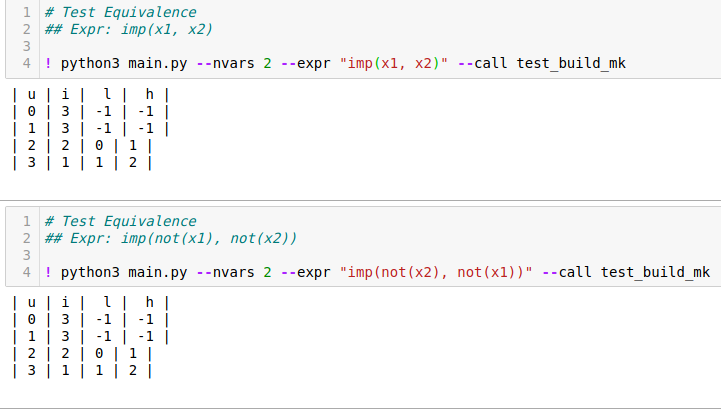
\includegraphics[height=200px, width=350px]{img/eq_check.png}
                \caption{Functional Equivalnce check}
                \label{fig:eq_check}
            \end{figure}

            It is evident that the two ROBDDs are equivalent thus verifying functional equivalence.
            This is because two different expressions always have unique ROBDDs.
            
            % The overall command for a particular instantiation with 7 variables is \\ $python3 main.py --nvars 7 --expr not(or(and(equiv(x1, x2), equiv(x3, x4)), or(equiv(imp(x1, x5), imp(x4, x6)), and(x3, x7)))) --nvars1 7 --expr1 and(equiv(x1, x2), equiv(x3, x4)) --nvars2 7 --expr2 or(equiv(imp(x1, x5), imp(x4, x6)), and(x3, x7)) --op or --j 2 --b 1 --call test_time_checks$

                        
            
    \section{References}

            [1]  \href{http://formal.cs.utah.edu:8080/pbl/BDD.php}{http://formal.cs.utah.edu:8080/pbl/BDD.php}
\end{document}